%#!platex --src-specials main.tex

\chapter{実験結果}
\label{chap:result}
本章では実験による結果を述べる. 
以下に各種次元削減を適用した1軸加速度触覚データと正規化を施した3軸加速度触覚データ, 無加工の3軸加速度触覚データを CNN で分類し, 出力から得られた4つの評価指標の値を以下の表\ref{tab:result}と図\ref{fig:accuracy}, \ref{fig:precision}, \ref{fig:recall}, \ref{fig:fmeasure}に示す. 

\begin{table}[htp]
\begin{center}
\caption{各データ処理手法に対する評価指標値}
\begin{tabular}{|c||c|c|c|c|}
\hline
data name           & accuracy & precision & recall & F-measure \\ \hline \hline
SA321-x             & 0.8571   & 0.8851    & 0.8571 & 0.8583    \\ \hline
SA321-y             & 0.8061   & 0.8384    & 0.8061 & 0.8020    \\ \hline
SA321-z             & 0.8163   & 0.7922    & 0.8163 & 0.7947    \\ \hline
SoC321              & 0.8367   & 0.8977    & 0.8367 & 0.8599    \\ \hline
Mag321              & 0.8673   & 0.9201    & 0.8673 & 0.8731    \\ \hline
PCA                 & 0.9184   & 0.9464    & 0.9184 & 0.9244    \\ \hline
DFT321              & 0.7653   & 0.9293    & 0.7653 & 0.8168    \\ \hline
original            & 0.9694   & 0.9767    & 0.9694 & 0.9694    \\ \hline
normalized original & 0.9184   & 0.9306    & 0.9184 & 0.9191    \\ \hline
\end{tabular}
\label{tab:result}
\end{center}
\end{table}

\begin{figure}[H]
    \begin{center}
    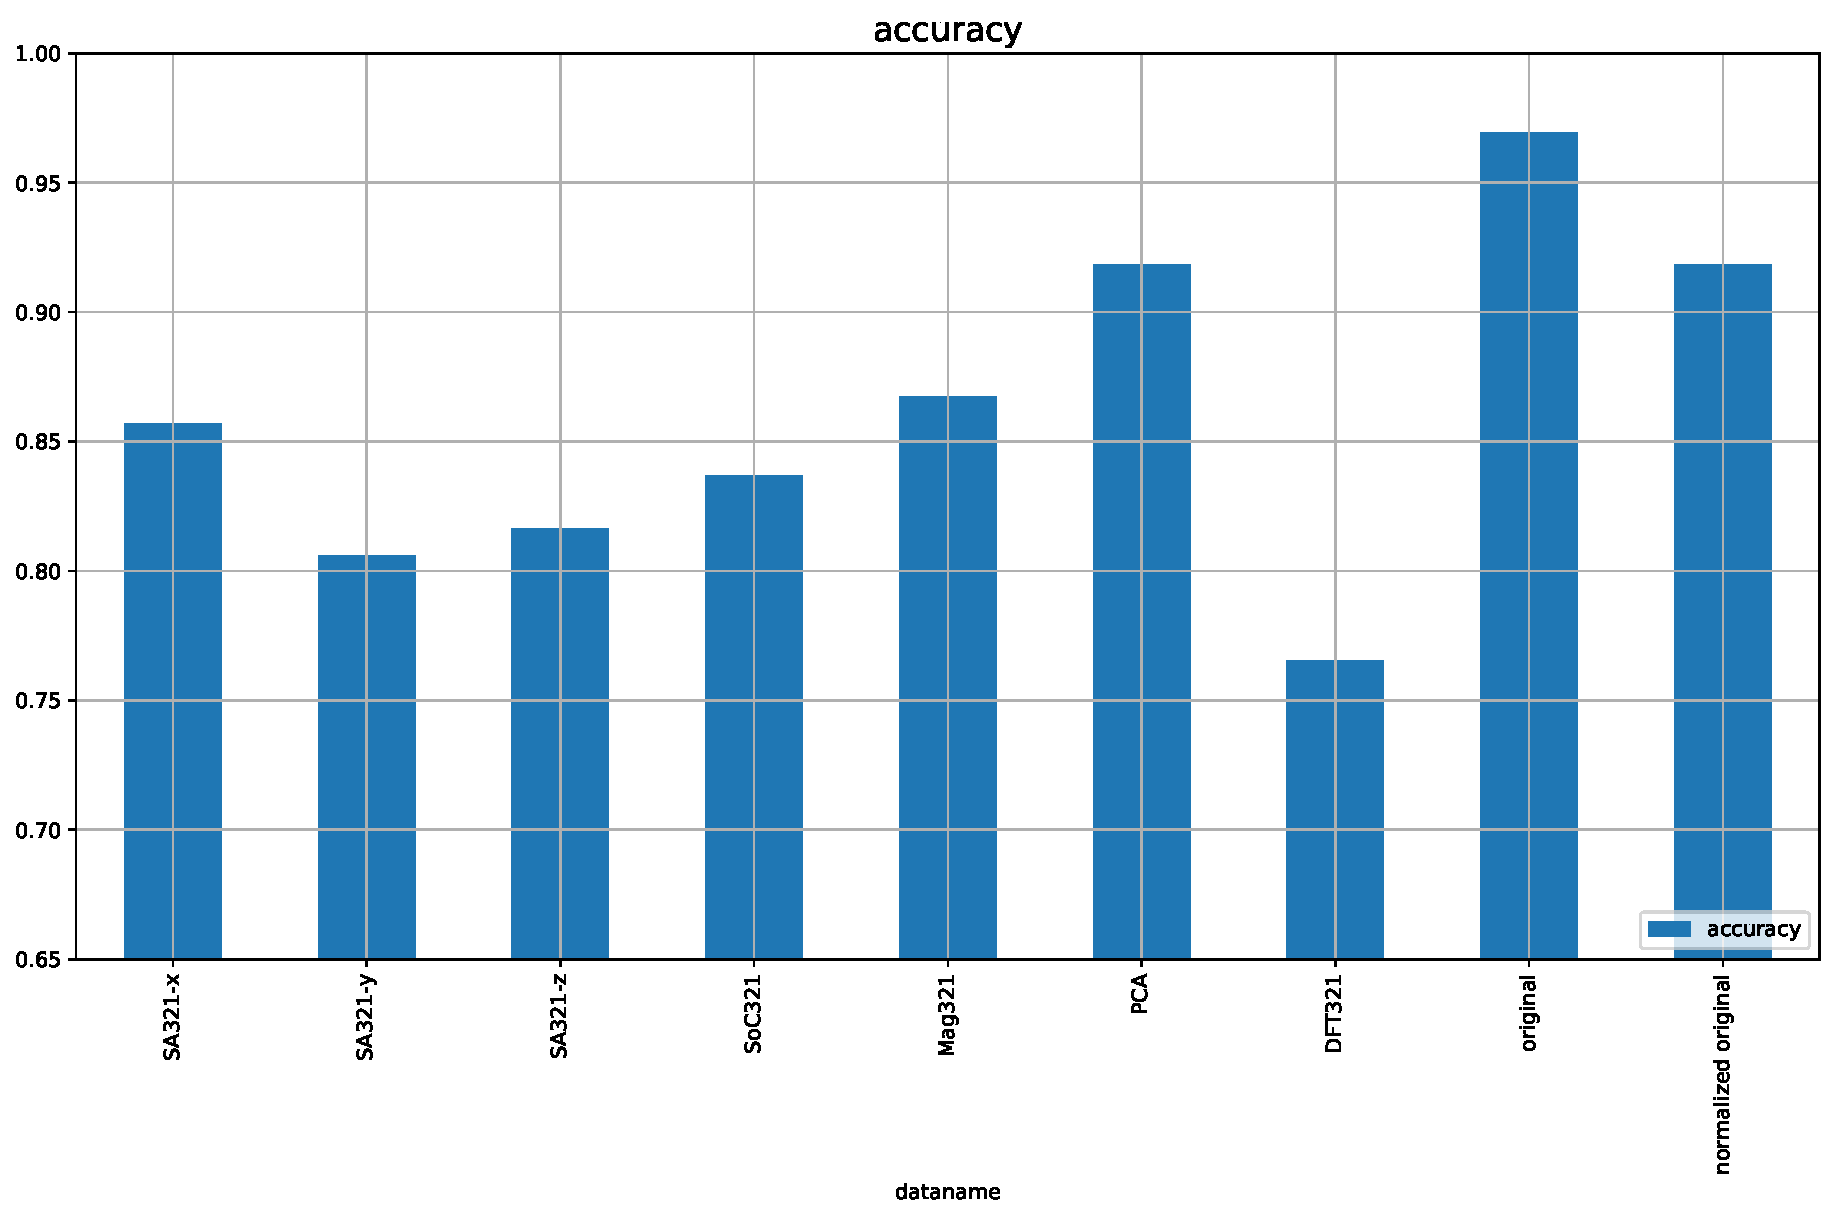
\includegraphics[width=12cm]{eps/accuracy.pdf}
    \caption{各データ処理手法に対する精度}
    \label{fig:accuracy}
   \end{center}
   \end{figure}
   
\begin{figure}[H]
    \begin{center}
    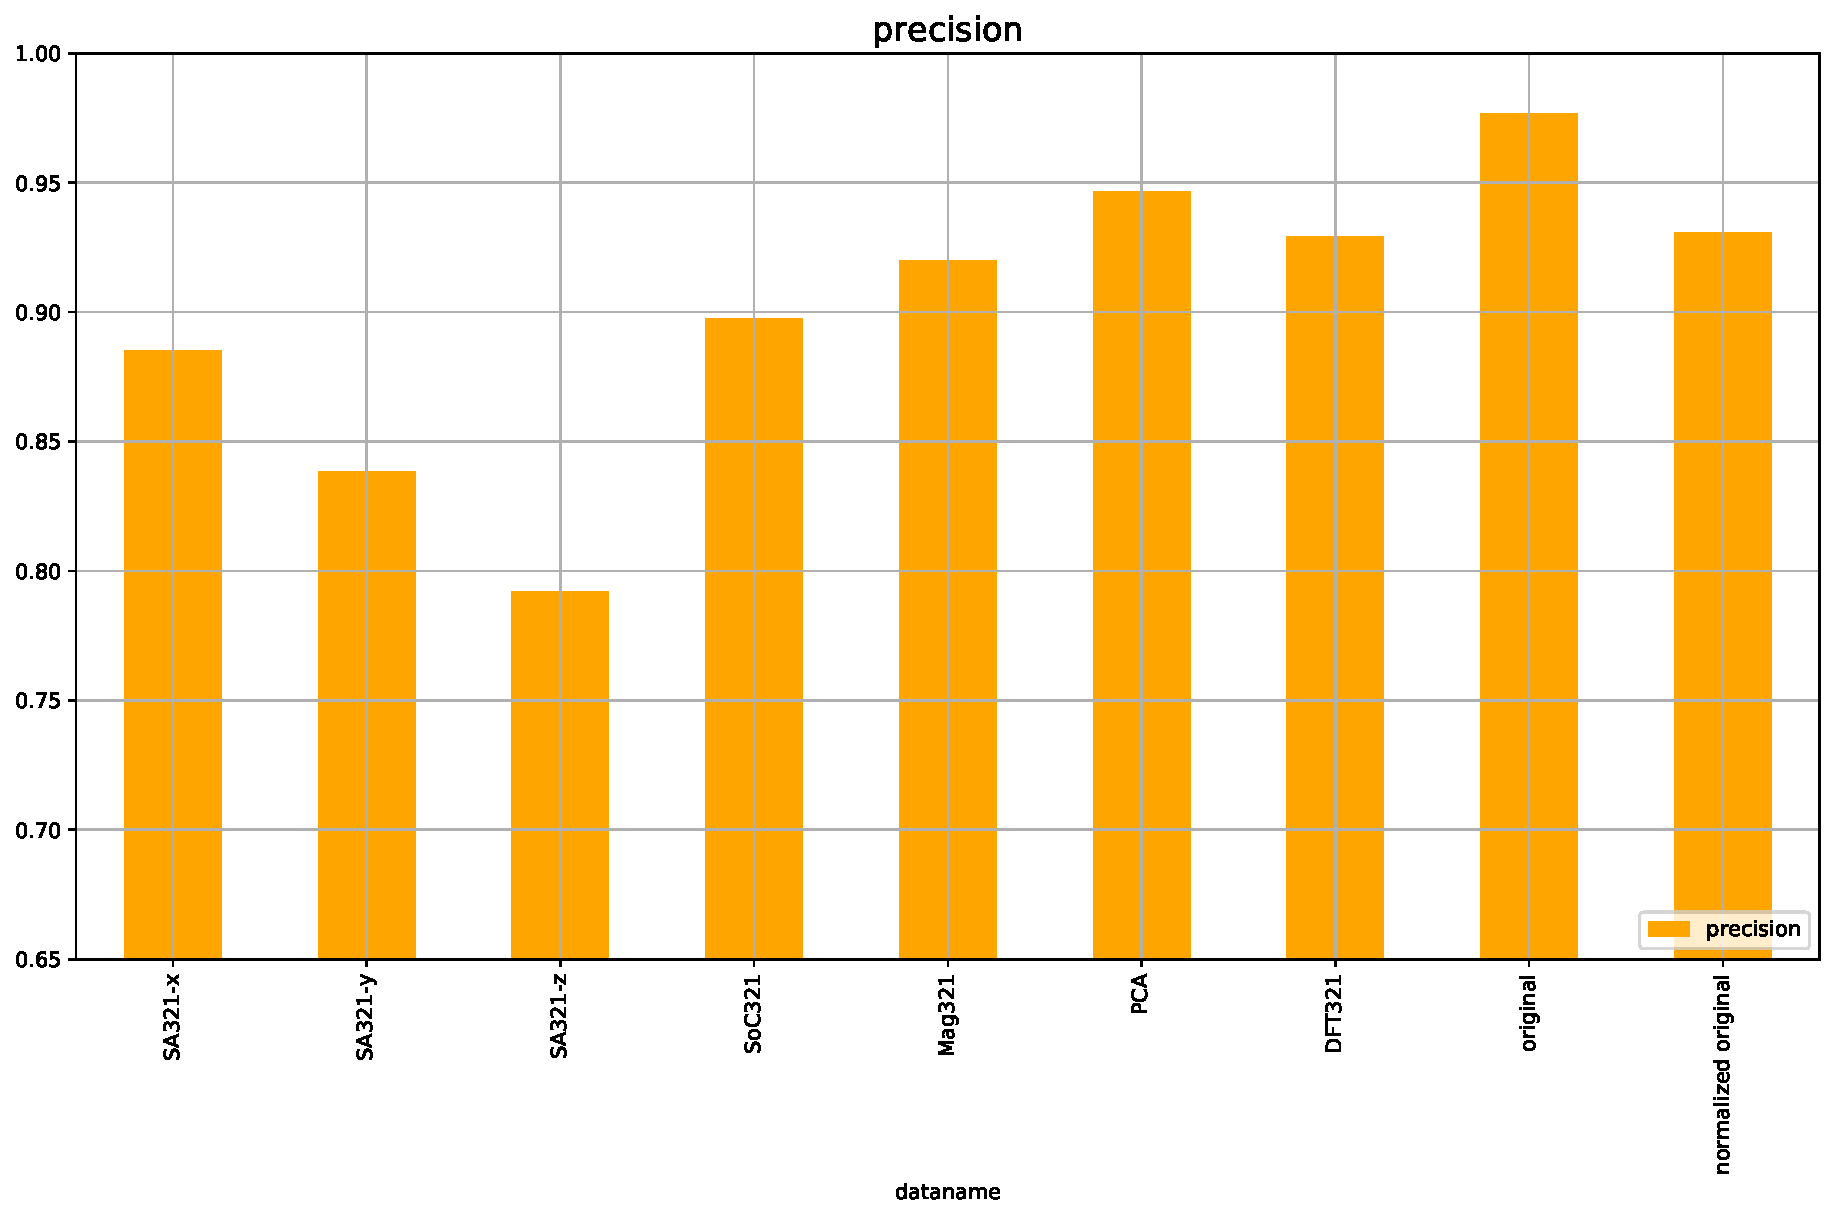
\includegraphics[width=12cm]{eps/precision.pdf}
    \caption{各データ処理手法に対する適合率}
    \label{fig:precision}
   \end{center}
   \end{figure}

\begin{figure}[H]
    \begin{center}
    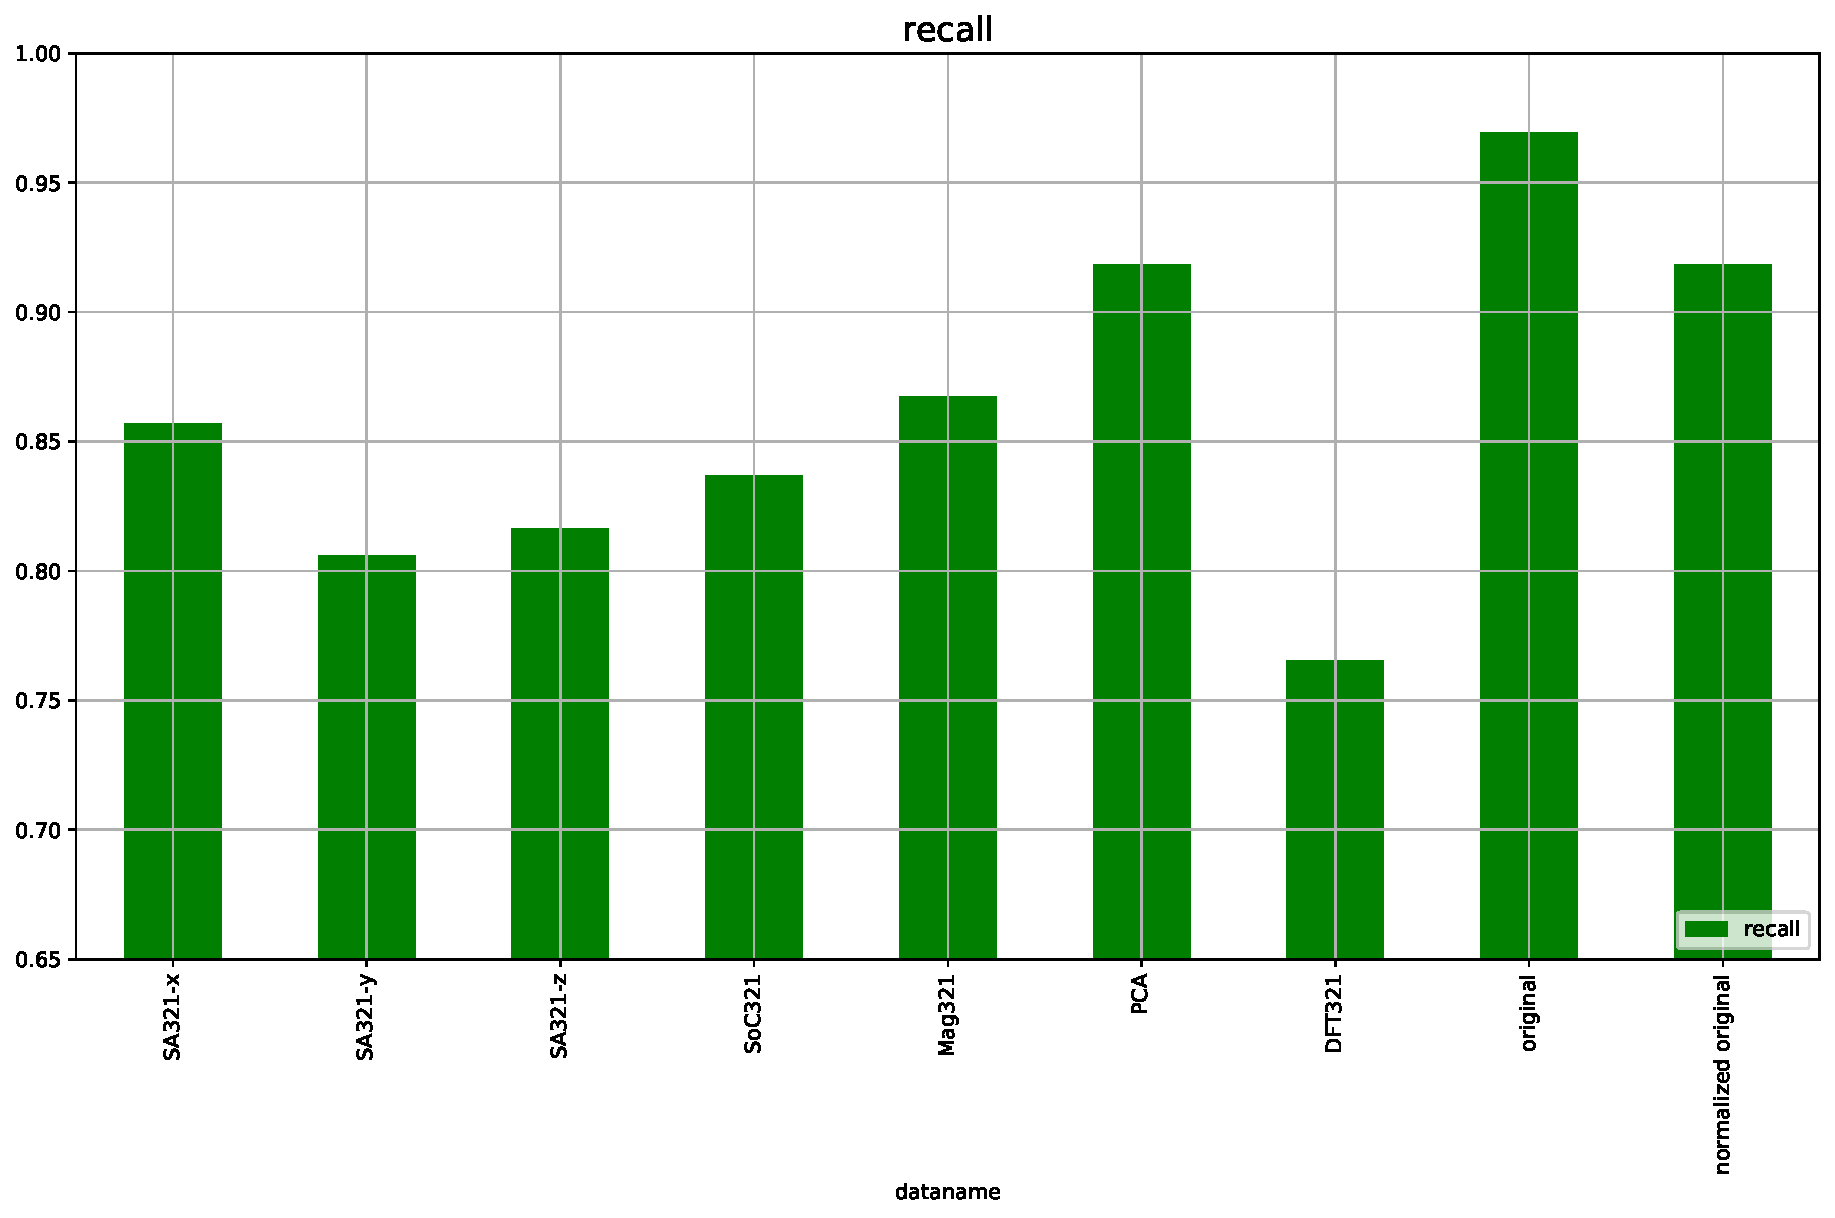
\includegraphics[width=12cm]{eps/recall.pdf}
    \caption{各データ処理手法に対する再現率}
    \label{fig:recall}
   \end{center}
   \end{figure}
   
\begin{figure}[H]
    \begin{center}
    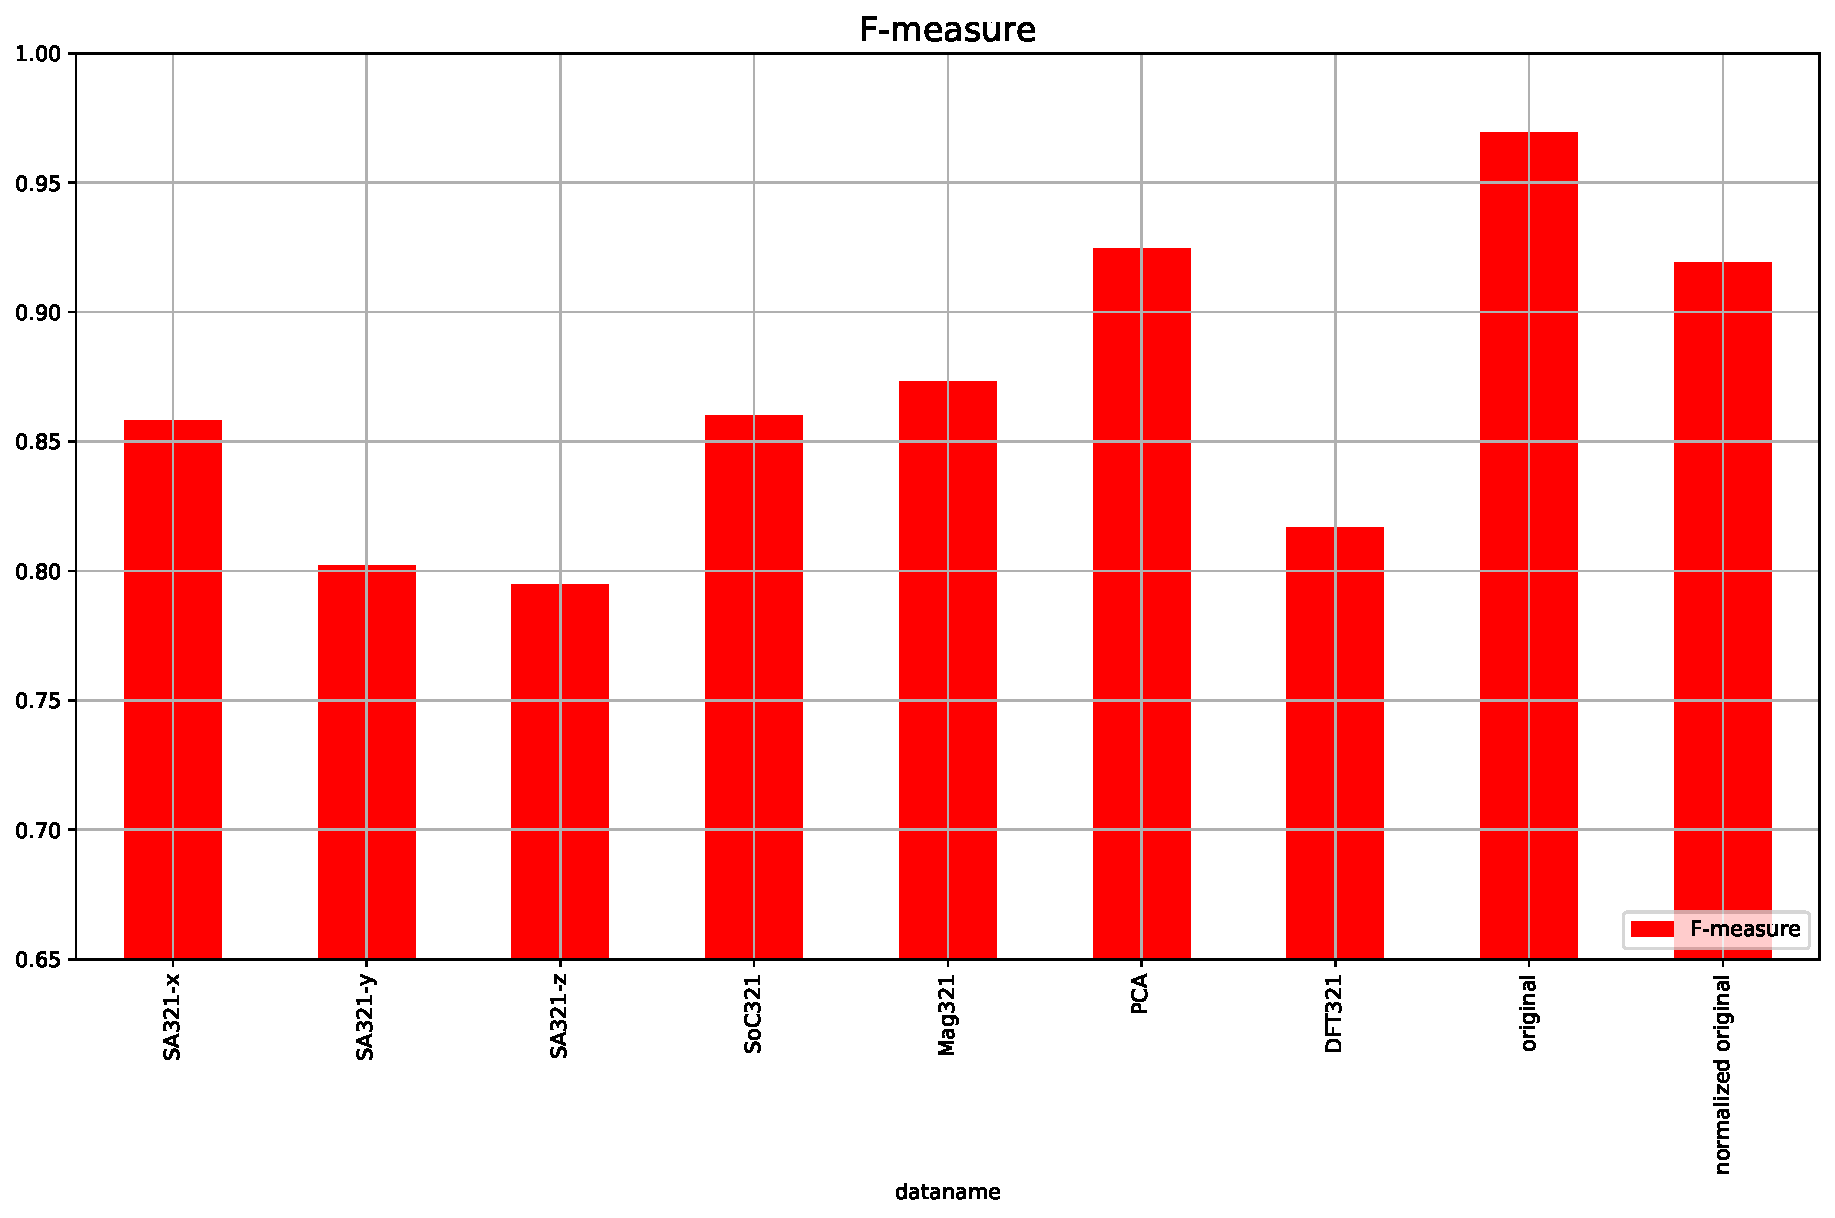
\includegraphics[width=12cm]{eps/F-measure.pdf}
    \caption{各データ処理手法に対するF値}
    \label{fig:fmeasure}
   \end{center}
   \end{figure}


% Local Variables:
% TeX-master: "main"
% mode: yatex
% End:
